\chapter{Statistical Inferences for Slopes}

\section{The Regression Model and Why We Need Inference for the Slope}

A sleep researcher pulls data from a sample of $8$ teenagers: daily screen time, in hours, and how many hours they slept that night. She plots the points, fits a line, and finds a slope of $b_1 = -0.16$: for every extra hour of screen time, sleep drops by about ten minutes. Does this mean the effect is real across all teenagers, or could a sample this size show a slope like this purely by chance, even if there is no relationship at all in the full population?

Recall from the Numerical Methods chapter that the least-squares regression line $\hat{y} = b_0 + b_1x$ is built entirely from your sample. You calculated $b_0$ and $b_1$, checked how well the line fit using $r$ and residuals, and used the line to predict $y$ for a given $x$. All of that was descriptive: a summary of the data you had in front of you.

But a sample slope is only one piece of evidence about a bigger question. Just as a sample proportion $\hat{p}$ estimates an unknown population proportion $p$, and a sample mean $\bar{x}$ estimates an unknown population mean $\mu$, a sample slope $b_1$ estimates an unknown population slope, written $\beta_1$. Statisticians describe the true relationship between two quantitative variables using a \newterm{population regression model}\index{population regression model}:
\[
Y = \beta_0 + \beta_1 X + \varepsilon
\]
Here $\beta_0$ is the population $y$-intercept, $\beta_1$ is the population slope, and $\varepsilon$ is a random error term: the part of $Y$ that isn't explained by $X$, capturing everything else that pushes an individual response above or below the line. $\beta_0$ and $\beta_1$ are parameters. They describe the entire population and, in practice, you never know their exact values. $b_0$ and $b_1$ are statistics, calculated from your one sample, and used to estimate $\beta_0$ and $\beta_1$.

This is exactly the same logic you used for proportions and means. There, you built confidence intervals and ran significance tests to reason from $\hat{p}$ to $p$, or from $\bar{x}$ to $\mu$. Now you will do the same thing for slopes: reason from $b_1$, the one number your sample happened to give you, to $\beta_1$, the value you actually care about.

\subsection*{Estimating the Slope and Intercept}

The formulas for $b_0$ and $b_1$ are the ones you already know:
\[
b_1 = r\frac{s_y}{s_x} \qquad \text{and} \qquad b_0 = \bar{y} - b_1\bar{x}
\]
where $r$ is the sample correlation coefficient and $s_x, s_y$ are the sample standard deviations of $X$ and $Y$. If you are working from raw sums instead of $r$, $s_x$, and $s_y$, an algebraically equivalent formula is
\[
b_1 = \frac{n\sum xy - \left(\sum x\right)\left(\sum y\right)}{n\sum x^2 - \left(\sum x\right)^2}
\]
Both formulas give the same $b_1$; use whichever matches the summary statistics you have on hand.

The residual for any data point is still $e = y - \hat{y}$, where $\hat{y} = b_0 + b_1x$ is the value your line predicts. The standard deviation of all the residuals in your sample, $s_e$, tells you the typical size of a prediction miss. You will lean on $s_e$ heavily in the next section, because it is the key ingredient in measuring how much $b_1$ itself might vary from sample to sample.

For the rest of this chapter, we will follow the sleep researcher's study. She samples $8$ teenagers at random and records their daily screen time ($X$, in hours) and their sleep duration that night ($Y$, in hours):

\begin{center}
\begin{tabular}{|c|c|c|c|c|c|c|c|c|}
\hline
Screen time (hr) & 2 & 3 & 4 & 5 & 6 & 7 & 8 & 9 \\
\hline
Sleep duration (hr) & 7.85 & 8.05 & 7.40 & 7.55 & 6.90 & 7.35 & 6.70 & 6.95 \\
\hline
\end{tabular}
\end{center}

For this sample, $\bar{x} = 5.5$, $\bar{y} = 7.34$, $s_x = 2.45$, $s_y = 0.47$, and $r = -0.854$. That gives
\[
b_1 = (-0.854)\frac{0.47}{2.45} = -0.165 \qquad b_0 = 7.34 - (-0.165)(5.5) = 8.25
\]
so $\hat{y} = 8.25 - 0.165x$. The negative slope matches what the researcher suspected: more screen time is associated with less sleep, at least in this sample. The question this chapter answers is whether that association is strong enough, and consistent enough, to conclude something about $\beta_1$ for teenagers in general, or whether a slope this far from zero is a believable result of sampling variation alone.

\begin{itemize}
    \item $Y = \beta_0 + \beta_1 X + \varepsilon$ is the population regression model; $\beta_0$ and $\beta_1$ are unknown parameters, and $\varepsilon$ is random error.
    \item $b_0$ and $b_1$ are sample statistics, calculated from your data, that estimate $\beta_0$ and $\beta_1$.
    \item $b_1 = r\dfrac{s_y}{s_x}$ and $b_0 = \bar{y} - b_1\bar{x}$, with an equivalent raw-sum formula available for $b_1$.
    \item The residual $e = y - \hat{y}$ and its standard deviation $s_e$ measure how far actual data points fall from the line.
\end{itemize}

\begin{Exercise}[title={Identifying the Model}, label={ex:slope-model-1}]
A horticulturist records the amount of fertilizer applied (in grams per plant) and the resulting plant height (in centimeters) for a random sample of tomato plants.
\begin{enumerate}
    \item Identify $X$ and $Y$ in this study.
    \item Write the population regression model for this relationship, using correct notation.
    \item In context, what would it mean if $\beta_1 = 0$?
    \item Explain why $\beta_1$ is not something the horticulturist can ever know exactly, even after collecting data from every plant she owns.
\end{enumerate}
\end{Exercise}

\begin{Answer}[ref={ex:slope-model-1}]
\begin{enumerate}
    \item $X$ is the amount of fertilizer applied (grams per plant); $Y$ is the resulting plant height (centimeters).
    \item $Y = \beta_0 + \beta_1 X + \varepsilon$, where $\beta_0$ is the population intercept, $\beta_1$ is the population slope relating fertilizer amount to height, and $\varepsilon$ is random error.
    \item If $\beta_1 = 0$, then fertilizer amount has no linear relationship with plant height in the population; the population regression line is flat, and knowing how much fertilizer a plant received tells you nothing about how tall it will grow.
    \item $\beta_1$ describes the relationship for the entire population of plants the horticulturist could ever grow, under all possible conditions, not just the ones she happened to collect data from. Even collecting data from every plant she currently owns would still leave $\beta_1$ unknown, since her plants are themselves a sample of all plants that could exist under those growing conditions. $\beta_1$ is a parameter; only a $b_1$ calculated from data is ever directly observed.
\end{enumerate}
\end{Answer}

\begin{Exercise}[title={Spot the Error}, label={ex:slope-model-2}]
A student in the sleep study writes: "I calculated $\beta_1 = -0.165$ from my sample of 8 teenagers, so I can conclude that increasing screen time by one hour causes a decrease of $0.165$ hours of sleep for every teenager." Identify two separate errors in this statement.
\end{Exercise}

\begin{Answer}[ref={ex:slope-model-2}]
First, the value $-0.165$ was calculated from the sample, so it should be labeled $b_1$, not $\beta_1$. $\beta_1$ refers to the unknown population slope; $b_1$ is the sample statistic used to estimate it. Second, the statement claims causation from an observational study. Unless screen time was randomly assigned to teenagers in an experiment, a relationship in the data does not establish that screen time causes reduced sleep. Other variables, such as stress or extracurricular schedules, could be influencing both screen time and sleep.
\end{Answer}

\begin{Exercise}[title={Computing the Line}, label={ex:slope-model-3}]
An engineer records the operating temperature (in degrees Celsius) and the battery life (in hours) for a random sample of $6$ devices. She finds $\bar{x} = 30$, $\bar{y} = 9.2$, $s_x = 8.5$, $s_y = 1.4$, and $r = -0.79$.
\begin{enumerate}
    \item Find $b_1$ and $b_0$.
    \item Write the least-squares regression equation.
    \item Predict the battery life for a device operating at $35^\circ$C.
\end{enumerate}
\end{Exercise}

\begin{Answer}[ref={ex:slope-model-3}]
\begin{enumerate}
    \item $b_1 = (-0.79)\dfrac{1.4}{8.5} = -0.130$; $b_0 = 9.2 - (-0.130)(30) = 13.10$.
    \item $\hat{y} = 13.10 - 0.130x$.
    \item At $x = 35$: $\hat{y} = 13.10 - 0.130(35) = 8.55$ hours.
\end{enumerate}
\end{Answer}

\textbf{Computing in Excel}

Enter the sleep study data from earlier in this section into two columns: screen time in cells A2 through A9, and sleep duration in cells B2 through B9, with headers in row 1.

\begin{enumerate}
    \item In an empty cell, enter \texttt{=SLOPE(B2:B9,A2:A9)}. Excel returns $-0.1649$, matching $b_1 = -0.165$ from the hand calculation (Excel simply keeps more decimal places).
    \item In another cell, enter \texttt{=INTERCEPT(B2:B9,A2:A9)}. Excel returns $8.2506$, matching $b_0 = 8.25$.
    \item To check the correlation behind the calculation, enter \texttt{=CORREL(A2:A9,B2:B9)}. Excel returns $-0.8536$, matching $r = -0.854$.
    \item To find $s_x$ and $s_y$ directly instead of computing them by hand, use \texttt{=STDEV.S(A2:A9)} and \texttt{=STDEV.S(B2:B9)}. These return $2.4495$ and $0.4732$.
\end{enumerate}

Watch the argument order: for both \texttt{SLOPE} and \texttt{INTERCEPT}, the known $y$-values are listed first, then the known $x$-values. Reversing the two ranges is a common mistake, and it will silently hand you the wrong sign or a nonsense intercept rather than an error message.

Exercise 3 gave you $\bar{x}$, $\bar{y}$, $s_x$, $s_y$, and $r$ directly rather than raw data, since with only five summary numbers, computing $b_1 = r\frac{s_y}{s_x}$ by hand is just as fast as opening a spreadsheet. \texttt{SLOPE} and \texttt{INTERCEPT} need the original data columns to work; if you had the original $6$ temperature and battery-life pairs instead, entering them into two columns and applying \texttt{SLOPE} and \texttt{INTERCEPT} directly would skip the $r$, $s_x$, $s_y$ step entirely.

% [placeholder: spreadsheet with screen time / sleep duration columns and SLOPE, INTERCEPT, CORREL formula results]

\section{The Sampling Distribution of $b_1$ and the Confidence Interval for the Slope}

Suppose the sleep researcher ran her study again with a brand new sample of $8$ teenagers. Would she get $b_1 = -0.165$ a second time? Almost certainly not exactly. A different sample means different data points, a different fitted line, and a different $b_1$. This is the same problem you have already run into twice before: a sample proportion $\hat{p}$ bounces around from sample to sample, and so does a sample mean $\bar{x}$. Now it is the slope's turn.

That variation is not a flaw in the method. It is exactly what a \newterm{sampling distribution}\index{sampling distribution!of the slope} describes: the distribution of $b_1$-values you would get if you repeated the study over and over, each time drawing a new random sample of the same size. Provided the conditions for inference hold (you will check these in detail in the next section), that sampling distribution of $b_1$ is approximately normal, centered at the true population slope $\beta_1$, with standard deviation $\sigma_{b_1}$.

In practice, you never know $\sigma_{b_1}$ exactly, because it depends on $\sigma_\varepsilon$, the population standard deviation of the errors, which is unknown. So you estimate it from your sample, calling the estimate $s_{b_1}$, the \newterm{standard error of the slope}\index{standard error!of the slope}. Once you replace the unknown $\sigma_{b_1}$ with the estimated $s_{b_1}$, the statistic
\[
t = \frac{b_1 - \beta_1}{s_{b_1}}
\]
no longer follows a normal distribution exactly. It follows a $t$-distribution with $df = n - 2$ degrees of freedom, the same pattern you saw for means: swap in an estimated standard error, lose a bit of precision, and the normal distribution becomes a $t$-distribution.

Here is a genuine difference from earlier chapters, though. For a proportion or a mean, you sometimes computed the standard error by hand from a simple formula. For the slope, you almost never will. $s_{b_1}$ depends on $s_e$, the sample size, and how spread out your $x$-values are, and computing it from scratch is tedious enough that no exam or workplace expects you to. Instead, $s_{b_1}$ is something you read directly from output, whether that is a graphing calculator's regression screen or software printout, in a column often labeled "StDev" or "SE Coef." Recognizing and interpreting that column, correctly, is itself a tested skill.

\subsection*{Constructing the Confidence Interval}

With $s_{b_1}$ in hand, a confidence interval for $\beta_1$ takes the same shape as every confidence interval you have built so far: statistic plus or minus a margin of error.
\[
\text{Margin of Error} = t^*s_{b_1} \qquad \text{Confidence Interval: } b_1 \pm t^*s_{b_1}
\]
where $t^*$ is the critical value from a $t$-distribution with $df = n-2$, chosen to match your desired confidence level.

Return to the sleep study. A statistical package fits the regression line to the $8$ data points and reports the following output:

\begin{center}
\begin{tabular}{|l|c|c|c|c|}
\hline
Predictor & Coef & StDev & T & P \\
\hline
Constant & 8.2506 & 0.2448 & 33.70 & 0.000 \\
Screen time & $-0.1649$ & 0.0411 & $-4.01$ & 0.007 \\
\hline
\end{tabular}
\end{center}

with $n = 8$, so $df = n - 2 = 6$. To build a $90\%$ confidence interval for $\beta_1$, look up $t^* = t_{0.05}(6) = 1.943$. Then
\[
\text{Margin of Error} = (1.943)(0.0411) = 0.0798
\]
\[
\text{Confidence Interval: } -0.1649 \pm 0.0798 = (-0.2447, -0.0850)
\]
We are $90\%$ confident that, for teenagers in general, each additional hour of daily screen time is associated with a change in average sleep duration of between $-0.245$ and $-0.085$ hours. Notice that this entire interval is negative. Since it does not contain $0$, every plausible value of $\beta_1$ in this interval represents some negative relationship between screen time and sleep, which is a first hint that the effect the researcher found in her sample may reflect something real in the population, and not just sampling noise. Sections 3 and 4 make that hint precise, first by checking whether this procedure was even valid to use, and then by testing the claim directly.

\begin{itemize}
    \item $b_1$ varies from sample to sample; its sampling distribution is centered at $\beta_1$ under the conditions for inference.
    \item The standard error $s_{b_1}$ is read directly from calculator or computer regression output; it is rarely computed by hand.
    \item $t = \dfrac{b_1 - \beta_1}{s_{b_1}}$ follows a $t$-distribution with $df = n - 2$.
    \item Confidence interval: $b_1 \pm t^*s_{b_1}$, with $t^*$ taken from the $t$-distribution at $df = n-2$.
    \item If a confidence interval for $\beta_1$ does not contain $0$, that is an early signal, not yet a conclusion, that the population slope may be nonzero.
\end{itemize}

\begin{Exercise}[title={Reading Computer Output}, label={ex:slope-ci-1}]
A researcher studies the relationship between weekly study hours ($X$) and the improvement in exam score, in points ($Y$), for a random sample of $n = 12$ students. Regression output gives $b_1 = 2.35$ and $s_{b_1} = 0.68$.
\begin{enumerate}
    \item Find the degrees of freedom for this problem.
    \item Construct a $95\%$ confidence interval for $\beta_1$. ($t^*_{0.025}(10) = 2.228$.)
    \item Interpret the interval in context.
\end{enumerate}
\end{Exercise}

\begin{Answer}[ref={ex:slope-ci-1}]
\begin{enumerate}
    \item $df = n - 2 = 12 - 2 = 10$.
    \item Margin of error $= (2.228)(0.68) = 1.515$. Confidence interval: $2.35 \pm 1.515 = (0.835, 3.865)$.
    \item We are $95\%$ confident that, in the population of students like those sampled, each additional hour of weekly study is associated with an average exam score improvement of between $0.835$ and $3.865$ points.
\end{enumerate}
\end{Answer}

\begin{Exercise}[title={Spot the Error}, label={ex:slope-ci-2}]
A student computes a $95\%$ confidence interval for the slope relating screen time and sleep duration and gets $(-0.265, -0.064)$. She writes: "There is a $95\%$ probability that the true slope $\beta_1$ falls between $-0.265$ and $-0.064$." Explain what is wrong with this interpretation and give a correct version.
\end{Exercise}

\begin{Answer}[ref={ex:slope-ci-2}]
$\beta_1$ is a fixed, though unknown, number; it either falls in that interval or it does not; there is no probability attached to it once the interval is calculated. The $95\%$ refers to the long-run success rate of the method: if we repeated this sampling process many times and built a confidence interval each time using the same procedure, about $95\%$ of those intervals would capture the true $\beta_1$. A correct interpretation is: "We are $95\%$ confident that the interval from $-0.265$ to $-0.064$ captures the true population slope $\beta_1$."
\end{Answer}

\begin{Exercise}[title={Fill In the Table}, label={ex:slope-ci-3}]
A separate study relates the number of hours of sleep lost the night before a road trip ($X$) to the number of driving errors made in a simulator ($Y$), for a random sample of $n = 11$ drivers. Regression output shows $b_1 = -4.8$ and $s_{b_1} = 1.5$.
\begin{enumerate}
    \item Find $df$ and the $t$-statistic for $b_1$.
    \item Construct a $90\%$ confidence interval for $\beta_1$. ($t^*_{0.05}(9) = 1.833$.)
    \item Does this interval suggest that sleep loss and driving errors are unrelated in the population? Explain using the interval.
\end{enumerate}
\end{Exercise}

\begin{Answer}[ref={ex:slope-ci-3}]
\begin{enumerate}
    \item $df = 11 - 2 = 9$. $t = \dfrac{-4.8}{1.5} = -3.20$.
    \item Margin of error $= (1.833)(1.5) = 2.750$. Confidence interval: $-4.8 \pm 2.750 = (-7.550, -2.050)$.
    \item No. The entire interval is negative and does not contain $0$, so every plausible value of $\beta_1$ represents a negative relationship between sleep loss and driving errors; this suggests the two are related in the population, not unrelated.
\end{enumerate}
\end{Answer}

%Check numbers again 

\textbf{Computing in Excel}

The regression output table above, including $s_{b_1}$, can be generated directly from the raw data rather than typed in by hand. Using the same screen time and sleep duration columns from Section 1 (A2:A9 and B2:B9):

\begin{enumerate}
    \item Select a blank $2 \times 2$ range, say D2:E3. Type \texttt{=LINEST(B2:B9,A2:A9,TRUE,TRUE)} and confirm with Ctrl+Shift+Enter (in newer versions of Excel with dynamic arrays, a plain Enter is enough). This fills all four cells at once:
    \begin{center}
    \begin{tabular}{|c|c|}
    \hline
    $b_1 = -0.1649$ & $b_0 = 8.2506$ \\
    \hline
    $s_{b_1} = 0.0411$ & $s_{b_0} = 0.2448$ \\
    \hline
    \end{tabular}
    \end{center}
    The top row gives the coefficients, in reverse order from how you might expect (slope first, then intercept); the row directly below gives each one's standard error.
    \item For the critical value, enter \texttt{=T.INV.2T(0.10,6)} in an empty cell. The first argument is $1 - \text{confidence level}$, and the second is $df = n - 2$. Excel returns $1.9432$, matching $t^*_{0.05}(6)$ from the table.
    \item Margin of error: reference the two cells you already have, \texttt{=D3*[t* cell]}, giving $0.0798$.
    \item Confidence interval bounds: \texttt{=D2-[margin cell]} and \texttt{=D2+[margin cell]}, giving $-0.2447$ and $-0.0850$.
\end{enumerate}

\texttt{LINEST} is the same idea as \texttt{SLOPE} and \texttt{INTERCEPT} from Section 1, but it returns the standard errors in the same step, so you never have to hunt for $s_{b_1}$ separately. The argument order is the same gotcha as before: known $y$'s first, known $x$'s second.

% [Screenshot placeholder: LINEST array output, T.INV.2T critical value, and CI computation for the sleep study data]

\section{Conditions for Inference on the Slope}

The confidence interval you just built in Section 2 quietly assumed something you have not actually checked yet: that it was valid to use a $t$-procedure at all. Every inference method in this book comes with conditions attached, and the slope is no exception. Skip the check, and a beautifully computed interval can still be meaningless.

You have already met four of these five conditions in some form, for proportions and for means. The fifth, linearity, is new, because it is specific to relationships between two variables rather than a single one.

\begin{itemize}
    \item \textbf{Random}: the data come from a random sample or a randomized experiment.
    \item \textbf{Linearity}: the true relationship between $X$ and $Y$ is actually linear, not curved.
    \item \textbf{Independence}: individual observations do not influence one another; if sampling without replacement, the population is at least $10$ times the sample size.
    \item \textbf{Normality}: for any fixed value of $X$, the residuals are approximately normally distributed.
    \item \textbf{Equal variance}: the spread of the residuals is roughly the same across all values of $X$.
\end{itemize}

Together these are sometimes remembered by the acronym LINER. Random and Independence are conditions you check from the design of the study itself, the same way you always have. Linearity, Normality, and Equal variance are different: you check all three using the same tool, a \newterm{residual plot}\index{residual plot}, which graphs each residual against its corresponding $x$-value.

A residual plot with no leftover curve supports linearity. A residual plot with a fairly even band of points, neither fanning out nor narrowing as $x$ increases, supports equal variance. And a roughly symmetric spread of residuals, without strong skew or outliers, supports normality, though a normal probability plot or a graph of the residuals alone gives a more direct check on shape than the residual-versus-$x$ plot does.

\subsection*{Checking the Conditions: The Sleep Study}

Return to the sleep researcher's $8$ teenagers. Before trusting the confidence interval from Section 2, check all five conditions.

\textbf{Random.} The researcher selected her $8$ teenagers using a random sampling method, so this condition is satisfied by the design of the study.

\textbf{Independence.} Teenagers in general form a population far larger than $8$, so sampling $8$ of them without replacement does not meaningfully affect the independence of their screen time or sleep duration from one another. The $10\%$ condition is easily satisfied.

\textbf{Linearity, Normality, and Equal variance.} These three come from the residuals themselves.

\begin{figure}[H]
\centering
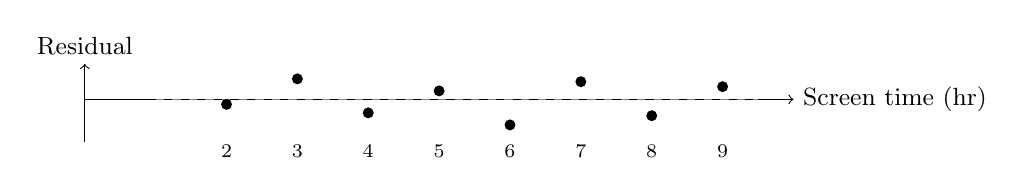
\begin{tikzpicture}[scale=0.9]
  \draw[->] (0,-0.6) -- (0,0.5) node[above] {\small Residual};
  \draw[->] (0,0) -- (10,0) node[right] {\small Screen time (hr)};
  \draw[dashed, gray] (1,0) -- (9.5,0);
  \foreach \x/\y in {2/-0.07, 3/0.29, 4/-0.19, 5/0.12, 6/-0.36, 7/0.25, 8/-0.23, 9/0.18} {
    \fill (\x,\y) circle (2.2pt);
  }
  \foreach \x in {2,3,4,5,6,7,8,9} {
    \node[below] at (\x,-0.5) {\scriptsize \x};
  }
\end{tikzpicture}
\caption{Residual plot for the sleep study regression.}
\label{fig:slope-resid-plot}
\end{figure}

The residuals in Figure \ref{fig:slope-resid-plot} bounce above and below $0$ with no visible curve, so linearity is reasonable: a straight line, rather than some curved model, is a sensible description of the relationship. The band of residuals also stays roughly the same width across the range of screen time values, from $2$ hours to $9$ hours, with no obvious funnel shape, so equal variance is reasonable as well.

\begin{figure}[H]
\centering
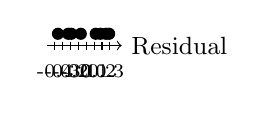
\begin{tikzpicture}[scale=1]
  \draw[->] (-0.5,0) -- (0.45,0) node[right] {\small Residual};
  \foreach \x in {-0.4,-0.3,-0.2,-0.1,0,0.1,0.2,0.3} {
     \draw (\x,-0.05) -- (\x,0.05);
     \node[below] at (\x,-0.12) {\scriptsize \x};
  }
  \foreach \x in {-0.36,-0.23,-0.19,-0.07,0.12,0.18,0.25,0.29} {
     \fill (\x,0.15) circle (2.2pt);
  }
\end{tikzpicture}
\caption{Dotplot of the eight residuals from the sleep study regression.}
\label{fig:slope-resid-dotplot}
\end{figure}

The dotplot in Figure \ref{fig:slope-resid-dotplot} shows no strong skew and no outliers among the eight residuals, so it is reasonable to proceed as though normality holds. With only $n = 8$ observations, though, this check is genuinely limited; a small sample simply does not give you enough information to rule out non-normality with much confidence. The honest conclusion is not "the residuals are normal," but "nothing in this small sample contradicts normality," which is a weaker, more defensible claim, and one that is worth stating explicitly on an exam or in a report.

With all five conditions reasonably satisfied, the confidence interval built in Section 2, and the hypothesis test coming in Section 4, both rest on solid ground.

\begin{itemize}
    \item The five conditions for slope inference: Random, Linearity, Independence, Normality, Equal variance (LINER).
    \item Random and Independence come from the design of the study.
    \item Linearity, Normality, and Equal variance are checked using a residual plot (and, for normality specifically, a dotplot, boxplot, or normal probability plot of the residuals).
    \item A small sample size limits how confidently you can assess normality; conclusions should be stated as "nothing contradicts" rather than "confirms."
\end{itemize}

\begin{Exercise}[title={Diagnosing a Residual Plot}, label={ex:slope-cond-1}]
A researcher studies the relationship between a car's weight and its fuel efficiency. The residual plot shows points that fan out widely for heavy cars but cluster tightly near $0$ for light cars.
\begin{enumerate}
    \item Which condition does this pattern call into question?
    \item Explain, in your own words, why this pattern is a problem for the validity of a confidence interval or test built from this data.
\end{enumerate}
\end{Exercise}

\begin{Answer}[ref={ex:slope-cond-1}]
\begin{enumerate}
    \item Equal variance. The spread of the residuals is clearly not constant across values of $X$; it grows as car weight increases.
    \item The standard error formula used to build $s_{b_1}$ assumes the same amount of scatter around the line at every value of $X$. If the scatter actually changes with $X$, as it does here, the standard error is not accurately estimated, so the resulting confidence interval and $p$-value cannot be trusted, even if every calculation is performed correctly.
\end{enumerate}
\end{Answer}

\begin{Exercise}[title={Checking Conditions in an Experiment}, label={ex:slope-cond-2}]
A greenhouse manager wants to know whether the amount of fertilizer given to a plant predicts its final height. She has $40$ identical seedlings and randomly assigns each one a fertilizer amount from a predetermined list of $8$ possible amounts, $5$ seedlings per amount. After eight weeks, she measures each plant's height and looks at the residual plot, which shows a fairly even, patternless band of points.
\begin{enumerate}
    \item Is the Random condition satisfied here? Explain, being careful about whether this is a sample or an experiment.
    \item Based on the residual plot description, which conditions does the data appear to satisfy?
\end{enumerate}
\end{Exercise}

\begin{Answer}[ref={ex:slope-cond-2}]
\begin{enumerate}
    \item Yes, though not through random sampling. This is a randomized experiment: fertilizer amounts were randomly assigned to seedlings, which satisfies the Random condition just as well as a random sample would for this purpose.
    \item A fairly even, patternless band of residuals supports linearity (no leftover curve) and equal variance (no fanning or narrowing). It does not, by itself, say anything about normality, which needs a separate look at the shape of the residuals rather than the pattern in a residual-versus-$x$ plot.
\end{enumerate}
\end{Answer}

\begin{Exercise}[title={Spot the Error}, label={ex:slope-cond-3}]
A student checking conditions for a slope inference problem writes: "I made a dotplot of the $x$-values and it looked roughly symmetric, so the Normality condition is satisfied." What is wrong with this reasoning?
\end{Exercise}

\begin{Answer}[ref={ex:slope-cond-3}]
The Normality condition is about the residuals, not the $x$-values. The distribution of the predictor variable itself does not need to be normal, and checking it tells you nothing about whether the errors around the regression line are normally distributed. The student should instead make a dotplot, boxplot, or normal probability plot of the residuals.
\end{Answer}

\section{Testing a Claim About the Slope}

The confidence interval in Section 2 hinted that the true slope $\beta_1$ is not $0$, since $(-0.2447, -0.0850)$ never crosses it. A hint is not a conclusion. To make the claim precise, and to attach an actual probability to the strength of the evidence, you need a significance test.

\subsection*{Step 1: State the Hypotheses}

The sleep researcher's original question was directional: does more screen time predict \emph{less} sleep, not just some unspecified difference. That points to a one-sided alternative.
\[
H_0: \beta_1 = 0 \qquad H_a: \beta_1 < 0
\]
$H_0$ says screen time has no linear relationship with sleep duration in the population of teenagers; $H_a$ says the relationship is negative. Use $\alpha = 0.05$.

\subsection*{Step 2: Name the Procedure and Verify Conditions}

Use a one-sample $t$-test for the slope of a regression line, with $df = n - 2$. Section 3 already checked all five conditions, Random, Linearity, Independence, Normality, and Equal variance, against this exact data set, and found no serious violations. Since the same data set is being reused here, that check still applies; there is no need to redo it.

\subsection*{Step 3: Calculate the Test Statistic and $P$-value}

Recall the regression output from Section 2:

\begin{center}
\begin{tabular}{|l|c|c|c|c|}
\hline
Predictor & Coef & StDev & T & P \\
\hline
Constant & 8.2506 & 0.2448 & 33.70 & 0.000 \\
Screen time & $-0.1649$ & 0.0411 & $-4.01$ & 0.007 \\
\hline
\end{tabular}
\end{center}

with $n = 8$, so $df = 6$. The test statistic is
\[
t = \frac{b_1 - 0}{s_{b_1}} = \frac{-0.1649}{0.0411} = -4.01
\]
matching the $T$ column exactly, since that column is always $\frac{\text{Coef}}{\text{StDev}}$.

The $P$ column, $0.007$, is a two-sided $p$-value: it treats $H_a: \beta_1 \ne 0$ as the alternative, whether or not that is the alternative you actually care about. Since our alternative here is one-sided, that number needs one adjustment before you can use it.

\begin{center}
\fbox{\begin{minipage}{0.9\textwidth}
\textbf{Converting a two-sided $p$-value to a one-sided $p$-value:}
\begin{enumerate}
    \item Check whether the sign of $t$ matches the direction claimed in $H_a$. Positive $t$ matches $H_a: \beta_1 > 0$; negative $t$ matches $H_a: \beta_1 < 0$.
    \item If the sign matches, divide the reported two-sided $p$-value by $2$.
    \item If the sign does not match, the data point the opposite way from your claim. The correct one-sided $p$-value is actually greater than $0.5$, no matter how small the two-sided number looks, and there is no evidence for $H_a$.
\end{enumerate}
\end{minipage}}
\end{center}

Here $t = -4.01$ is negative, matching the direction of $H_a: \beta_1 < 0$, so the sign check passes. The one-sided $p$-value is
\[
p\text{-value} = \frac{0.007}{2} = 0.0035
\]

\subsection*{Step 4: State a Conclusion}

Because $p = 0.0035 < \alpha = 0.05$, reject $H_0$. There is convincing statistical evidence that, in the population of teenagers this sample represents, more daily screen time is associated with a decrease in average nightly sleep duration. Because the screen time data were observed rather than randomly assigned, this conclusion is about association, not causation; some other factor could plausibly be driving both variables at once.

\begin{itemize}
    \item Test statistic: $t = \dfrac{b_1 - 0}{s_{b_1}}$, with $df = n - 2$, using the value of $\beta_1$ specified in $H_0$ (usually $0$).
    \item Standard computer output typically reports a two-sided $p$-value by default, regardless of which alternative you are actually testing.
    \item For a one-sided $H_a$, divide the reported two-sided $p$-value by $2$ only if the sign of $t$ matches the direction of $H_a$; otherwise the true one-sided $p$-value exceeds $0.5$.
    \item Reject $H_0$ when $p < \alpha$; state the conclusion in context, and be careful not to claim causation from an observational study.
\end{itemize}

\begin{Exercise}[title={Running the Test}, label={ex:slope-test-1}]
A marketing analyst studies the relationship between weekly advertising spend, in thousands of dollars ($X$), and weekly sales, in thousands of dollars ($Y$), for a random sample of $n = 10$ stores. She expects that more spend predicts more sales. Regression output gives $b_1 = 3.6$ and $s_{b_1} = 1.2$.
\begin{enumerate}
    \item State $H_0$ and $H_a$.
    \item Find $df$ and the test statistic $t$.
    \item Software reports a two-sided $p$-value of $0.0171$. Find the correct one-sided $p$-value.
    \item At $\alpha = 0.05$, state a conclusion in context.
\end{enumerate}
\end{Exercise}

\begin{Answer}[ref={ex:slope-test-1}]
\begin{enumerate}
    \item $H_0: \beta_1 = 0$; $H_a: \beta_1 > 0$.
    \item $df = 10 - 2 = 8$. $t = \dfrac{3.6}{1.2} = 3.00$.
    \item $t = 3.00$ is positive, matching the direction of $H_a: \beta_1 > 0$, so the sign check passes. One-sided $p$-value $= \dfrac{0.0171}{2} = 0.0086$.
    \item Since $p = 0.0086 < \alpha = 0.05$, reject $H_0$. There is convincing statistical evidence that, among stores like those sampled, higher advertising spend is associated with higher weekly sales.
\end{enumerate}
\end{Answer}

\begin{Exercise}[title={Spot the Error}, label={ex:slope-test-2}]
A student is testing $H_0: \beta_1 = 0$ against $H_a: \beta_1 < 0$ for a study relating hours of television watched to standardized test scores. Regression output gives $t = 2.10$ and a two-sided $p$-value of $0.0575$. The student writes: "The one-sided $p$-value is $0.0575 / 2 = 0.0288$, which is less than $0.05$, so I reject $H_0$ and conclude there is a negative relationship." Identify the error and give the correct one-sided $p$-value.
\end{Exercise}

\begin{Answer}[ref={ex:slope-test-2}]
The student divided the two-sided $p$-value by $2$ without first checking whether the sign of $t$ matches the direction of $H_a$. Here $t = 2.10$ is positive, but $H_a$ claims a negative relationship ($\beta_1 < 0$); the sign does not match. This means the sample data actually point in the opposite direction from what $H_a$ claims, so the correct one-sided $p$-value is not $0.0288$, but $1 - 0.0288 = 0.9712$, which is far from significant. There is no evidence here of a negative relationship; if anything, the (non-significant) trend runs the other way.
\end{Answer}

\begin{Exercise}[title={Interpreting the Conclusion}, label={ex:slope-test-3}]
Using the sleep study results from this section ($p = 0.0035$, $\alpha = 0.05$), a classmate says: "This proves that screen time causes reduced sleep in teenagers." Explain what is wrong with this statement, and rewrite it as a statistically defensible conclusion.
\end{Exercise}

\begin{Answer}[ref={ex:slope-test-3}]
The word "proves" overstates what a significance test can show; a small $p$-value provides convincing evidence against $H_0$, not proof. More importantly, the study is observational, since screen time was not randomly assigned to the teenagers. Without random assignment, a demonstrated relationship cannot establish causation; some other variable, such as stress level, extracurricular commitments, or household routines, could be influencing both screen time and sleep duration. A defensible conclusion: "There is convincing statistical evidence of a negative association between screen time and sleep duration in this population, but since the study was observational, this does not establish that screen time causes reduced sleep."
\end{Answer}

\textbf{Computing in Excel}

Continuing from the \texttt{LINEST} output in Section 2 (cell D2 for $b_1$, cell D3 for $s_{b_1}$):

\begin{enumerate}
    \item Test statistic: in an empty cell, enter \texttt{=D2/D3}. Excel returns $-4.0131$, matching the $T$ column of the regression output.
    \item One-sided $p$-value directly: enter \texttt{=T.DIST(D2/D3,6,TRUE)}. This gives the left-tail probability $P(T < t)$ for $df = 6$, which is exactly the one-sided $p$-value for $H_a: \beta_1 < 0$ when $t$ is negative. Excel returns $0.0035$, with no separate halving step needed.
    \item If you only have the two-sided $p$-value from a printed output table, use \texttt{=T.DIST.2T(ABS(D2/D3),6)/2} instead, which reproduces the halving rule from Step 3 directly. Both approaches agree here: $0.0035$.
\end{enumerate}

\texttt{T.DIST} assumes a lower-tail test by default; for $H_a: \beta_1 > 0$, use \texttt{=1-T.DIST(t,df,TRUE)} or the equivalent \texttt{=T.DIST.RT(t,df)} instead, since you need the upper tail.

% [Screenshot placeholder: T.DIST and T.DIST.2T formulas computing the one-sided p-value for the sleep study]

\textbf{Computing in Python}

The full test, from raw data to conclusion, takes only a few lines with \mintinline{python}{scipy.stats}:

\begin{minted}{python}
import numpy as np
from scipy import stats

x = np.array([2, 3, 4, 5, 6, 7, 8, 9])
y = np.array([7.85, 8.05, 7.40, 7.55, 6.90, 7.35, 6.70, 6.95])

result = stats.linregress(x, y)
df = len(x) - 2
t_stat = result.slope / result.stderr
p_one_sided = stats.t.cdf(t_stat, df)   # left tail, for Ha: beta1 < 0

print(f"b1 = {result.slope:.4f}, SE(b1) = {result.stderr:.4f}")
print(f"t = {t_stat:.4f}, df = {df}")
print(f"one-sided p-value = {p_one_sided:.4f}")
\end{minted}

This prints \mintinline{python}{b1 = -0.1649, SE(b1) = 0.0411}, \mintinline{python}{t = -4.0131, df = 6}, and \mintinline{python}{one-sided p-value = 0.0035}, matching the by-hand and Excel results exactly. \mintinline{python}{stats.t.cdf(t_stat, df)} gives the lower-tail probability directly, which is the correct one-sided $p$-value whenever $H_a$ is "less than and $t$ is negative; for a "greater than" alternative, use \mintinline{python}{1 - stats.t.cdf(t_stat, df)} instead.

